\section{Resultate \& Ausblick}\label{sec:conflict}

Nachfolgend vergleicht man die drei Dimensionen für die drei verschiedenen Szenarien.

\paragraph{Wirtschaft}
Wirtschaftlich betrachtet haben wir die Situation für das Jahr 2013 mit einer 6
bewertet. Die Innovation sowie die Anzahl Arbeitsplätze profitieren immer noch von
der nachsteigenden Nachfrage nach Tantal. Dieser anhaltende Anstieg hat bis 2035 zur Folge,
dass zwar weitere Arbeitsplätze entstehen, jedoch aber auch der Preis sich stark erhöhen
wird. Bezüglich Innovation sind keine Veränderungen ersichtlich. Auf aktuellen Prognosen
basierend haben wir somit die zu erwartende Situation bis 2035 weniger nachhaltig mit einer 5 eingestuft.
Im Alternativszenario steigt die Nachfrage nach Tantal weniger stark an. Somit werden
weniger neue Arbeitsplätze entstehen, der Preis wird nicht so drastisch ansteigen
und die Alternativtechnologie kann die Innovation stark antreiben. Dieses Szenario
erhält somit eine 6\(\frac{1}{3}\) und ist somit nachhaltiger als die Situation
im Jahr 2013.

\paragraph{Umwelt}
Die weltweite Nutzung von Tantal bewerten wir für das Jahr 2013 aus ökologischer
Sicht als neutral (5 auf der Skala). Dabei heben sich die geringen direkten
Folgen der Tantalgewinnung und die gravierenden Konsequenzen für den Naturraum
auf, während der Verbrauch als solches ebenfalls als neutral eingeschätzt wird.
Bei einem anhaltenden Trend und der damit einhergehenden Steigerung der
Fördermenge verschlechtern sich die Werte der einzelnen Indikatoren bis 2035 zum
Teil massiv. Speziell der Rohstoffverbrauch und die daraus resultierende
Verminderung des Rohstoffbestandes haben schwerwiegende Folgen. Durch die
Einführung einer neuen Technologie zur Herstellung von Kondensatoren könnte die
Nachfrage hochgerechnet um 40\% gesenkt werden. Da jedoch davon ausgegangen
wird, dass bis 2035 mehr als doppelt so viel Tantal benötigt wird, reicht
diese Massnahme alleine nicht, um zumindest auf dem gleichen Niveau zu bleiben
wie 2013. 

\paragraph{Gesellschaft}
Die gesellschaftliche Nachhaltigkeit für das Jahr 2013 wird mit 4\(\frac{1}{4}\) als negativ
bewertet. Begründet wird dies mit der Tatsache, dass ein bedeutender Anteil der
globalen Tantalgewinnung in Konfliktgebieten stattfindet. Die prognostizierte 
Steigerung der Nachfrage bis 2035 führt mit einer Bewertung von 5 zu einer 
Besserung gegenüber 2013. Sofern die Massnahmen zur Kontrolle von Konfliktmineralien 
Wirkung zeigen und die gesteigerte Nachfrage zu mehr Arbeitsplätzen führt. Falls bis
2035 eine Alternative zu Tantal eingeführt wird, wirkt sich dies negativ auf die 
Nachhaltigkeit aus. Einerseits führt dies zum Verlust von Arbeitsplätzen in Regionen
mit bereits sehr hoher Arbeitslosigkeit, andererseits wird angenommen, dass der 
Fokus in Konfliktgebieten auf andere Mineralien wie Gold gelegt wird. Der erhöhte Druck
auf den Goldabbau fördert wiederum Konflikte um die Kontrolle der Ressourcen. Daher 
wird dieses Szenario mit 3\(\frac{1}{2}\) bewertet.


\begin{center}
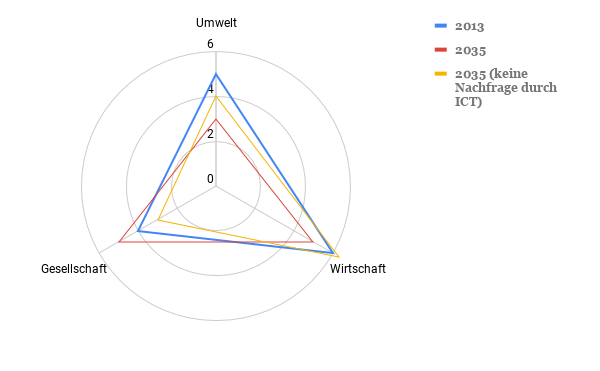
\includegraphics[width=14cm]{images/tantal-results}
\captionof{figure}{Vergleich der Nachhaltigkeit der drei verschiedenen Szenarien.}
\end{center}
